\chapter{Metody statystyczne} \label{ch5}

\section{Względna pozycja głowy członu}

\begin{table}[H]
\centering
\begin{tabular}{lrrrrrrrr}
  \toprule
Język & \multicolumn{4}{c}{lewy człon} & \multicolumn{4}{c}{prawy człon}\\
 & \multicolumn{1}{c}{N} & \multicolumn{1}{c}{średnia} & \multicolumn{1}{c}{t} & \multicolumn{1}{c}{p} & \multicolumn{1}{c}{N} & \multicolumn{1}{c}{średnia} & \multicolumn{1}{c}{t} & \multicolumn{1}{c}{p} \\ 
  \midrule
  \multicolumn{9}{c}{\textbf{Języki inicjalne}} \\
  \midrule
  angielski 	& 12326 	& \textbf{0,36} & $-$37 & 1.74e$-$288 & 15155 & \textbf{0,40} & $-$31 & 1.99e$-$199 \\
  czeski 	& 51416 	& \textbf{0,34} & $-$88 & 0 		& 62872 & \textbf{0,39} & $-$70 & 0 \\ 
  hiszpański	& 19685 & \textbf{0,30} & $-$74 & 0 		& 22137 & \textbf{0,31} & $-$80 & 0 \\ 
  islandzki 	& 31929 	& \textbf{0,18} & $-$196 & 0 		& 36967 & \textbf{0,18} & $-$225 & 0 \\ 
  polski 	& 9976 	& \textbf{0,23} & $-$74 & 0 		& 12049 & \textbf{0,33} & $-$50 & 0 \\ 
  portugalski & 19732 & \textbf{0,30} & $-$71 & 0 		& 22349 & \textbf{0,30} & $-$84 & 0 \\ 
  rosyjski 	& 36608 	& \textbf{0,38} & $-$56 & 0 		& 46050 & \textbf{0,41} & $-$47 & 0 \\ 
  rumuński 	& 27224 	& \textbf{0,37} & $-$53 & 0 		& 31024 & \textbf{0,37} & $-$60 & 0 \\ 
  włoski 	& 17728 	& \textbf{0,43} & $-$22 & 1,2e$-$107	& 20330 & \textbf{0,37} & $-$49 & 0 \\
  \midrule
  \multicolumn{9}{c}{\textbf{Języki mieszane}} \\
  \midrule
  łaciński 	& 19766 & \textbf{0,36}	& $-$47 & 0 		& 25755 & \textbf{0,48} & $-$5,8 & 7,98e$-$09 \\
  niemiecki & 51068 	& \textbf{0,53}	& 17 & 9,27e$-$62	& 64616 & \textbf{0,52} & 14 & 2,61e$-$46 \\ 
  \midrule
  \multicolumn{9}{c}{\textbf{Języki finalne}} \\
  \midrule
  koreański	& 6801 & \textbf{0,78} & 59 & 0 			& 12951 & \textbf{0,65} & 47 & 0 \\ 
  turecki 	& 7994 & \textbf{0,64} & 28 & 7,97e$-$167	& 12763 & \textbf{0,69} & 55 & 0 \\
  \bottomrule
\end{tabular}
\caption{Względna pozycja głów członów koordynacji}
\label{tab:pozycja-głowy}
\end{table}



Tabela \ref{tab:pozycja-głowy} przedstawia rozkład względnej pozycji głowy członów w~obrębie prawych i~lewych członów w~różnych językach. Pod uwagę brane są człony, których głowa nie jest jedynym elementem (tj. takie, które mają przynajmniej dwa tokeny). Pozycja głowy członu ustalana jest na podstawie następującego wzoru:

\[
P = \frac{H-1}{N-1} \text{ dla } N\geq2, \text{ gdzie:}
\]

\begin{itemize}
\item $P$ oznacza względną pozycję głowy członu w~członie;
\item $H$ oznacza pozycję głowy członu w~członie;
\item $N$ oznacza długość członu w~tokenach.
\end{itemize}

W przykładzie \eqref{numery} głowa lewego członu \textit{Urząd} znajduje się na samym początku członu, czyli w~pozycji $P=\frac{1-1}{2-1}=0$, zaś głowa prawego członu \textit{Izba} na jego środku, czyli w~pozycji $P=\frac{2-1}{3-1}=0{,}5$.

\begin{exe}
\ex \label{numery}
\begin{dependency}[theme=simple, baseline=0.5ex]
\begin{deptext}
\textbf{Urząd} \& Skarbowy \& i \& Krajowa \& \textbf{Izba} \&  Rozliczeniowa \\
\scriptsize \textbf{1} \& \scriptsize 2 \&   \& \scriptsize 1 \& \scriptsize \textbf{2} \& \scriptsize 3 \\
\end{deptext}
\wordgroup{1}{1}{2}{L}
\wordgroup{1}{4}{6}{R}
\end{dependency}
\end{exe}

W~językach inicjalnych głowa członu występuje znacznie częściej na początku członu ($<0{,}5$), zaś w~językach inicjalnych częściej na jego końcu ($>0{,}5$). Dotyczy to zarówno lewych, jak i~prawych członów koordynacji.

W przypadku języków mieszanych nie można zaobserwować wyraźnej prawidłowości. W~łacinie głowy lewych członów znajdują się częściej bliżej początku członu, zaś głowy prawych członów bliżej środka członu. W~języku niemieckim głowy członów są w~okolicach środka członu. Z tego powodu w~dyskusji wyników nie interpretuję wyników dla języków mieszanych w~kontekście przewidywań dotyczących struktury zależnościowej koordynacji.

Istotność statystyczna uzyskanych wyników jest potwierdzona testem t-Studenta sprawdzającym różność pozycji głowy od $0{,}5$, czyli środka członu\footnote{
Do analizy statystycznej użyto funkcji \texttt{t.test} języka R. Ilekroć w~niniejszej pracy występuje p = 0, przez 0 należy rozumieć liczbę dodatnią mniejszą od \texttt{Mashine\$double.xmin} $\approx 5e-324$ \citep{R2023}.}.

\section{Pozycja nadrzędnika}

Tabela \ref{tab:pozycja-nadrzędnika} pokazuje rozkład występowania koordynacji o różnych pozycjach nadrzędnika w~zależności od języka\footnote{
Do wszystkich koordynacji należą również te z~nadrzędnikiem po środku (M).}.

\begin{table}[h]
\centering
\begin{tabular}{lrrrrrrr}
  \toprule
& \multicolumn{1}{c}{Wszystkie}	& \multicolumn{4}{c}{Nadrzędnik po} 	& \multicolumn{2}{c}{Brak} \\
\multicolumn{1}{c}{Język}	& \multicolumn{1}{c}{koordynacje}	
& \multicolumn{2}{c}{lewej}			& \multicolumn{2}{c}{prawej}	& \multicolumn{2}{c}{nadrzędnika} \\
& \multicolumn{1}{c}{N} & 
\multicolumn{1}{c}{N} & \multicolumn{1}{c}{P} & \multicolumn{1}{c}{N} &
\multicolumn{1}{c}{P} & \multicolumn{1}{c}{N} & \multicolumn{1}{c}{P} \\
\midrule
\multicolumn{8}{c}{Języki inicjalne} \\
\midrule
angielski 	& 21013 & 11171 & \textbf{0.53} & 2972  & 0.14 & 6829  & 0.32 \\
czeski 		& 90566 & 49341 & \textbf{0.54} & 14279 & 0.16 & 26688 & 0.29 \\ 
hiszpański	& 28666 & 19557 & \textbf{0.68} & 2751  & 0.10 & 6300  & 0.22 \\ 
polski 		& 16684 & 8407  & \textbf{0.50} & 2219  & 0.13 & 6023  & 0.36 \\ 
portugalski 	& 29255 & 17661 & \textbf{0.60} & 3157  & 0.11 & 8364  & 0.29 \\  
rosyjski		& 61004 & 31679 & \textbf{0.52} & 8485  & 0.14 & 20556 & 0.34 \\ 
rumuński 	& 37247 & 21873 & \textbf{0.59} & 3088  & 0.08 & 11993 & 0.32 \\
włoski		& 25426 & 17014 & \textbf{0.67} & 2345  & 0.09 & 5992  & 0.24 \\ 
\hdashline 
islandzki 	& 43852 & 16986 & 0.39 & 2928 & 0.07 & 23877 & \textbf{0.54} \\ 
\midrule
\multicolumn{8}{c}{Języki mieszane} \\
\midrule
łacina 		& 39510 & 19635 & \textbf{0.50} & 9264  & \textbf{0.23} & 9112  & 0.23 \\ 
niemiecki 	& 92115 & 43089 & \textbf{0.47} & 23637 & \textbf{0.26} & 24029 & 0.26 \\ 
\midrule
\multicolumn{8}{c}{Języki finalne} \\
\midrule
koreański	& 21506 & 718   & 0.03 & 14289 & \textbf{0.66} & 6491 & 0.30 \\ 
turecki		& 19598 & 1760  & 0.09 & 11936 & \textbf{0.61} & 5758 & 0.29 \\ 
\bottomrule
\end{tabular}
\caption{Pozycja nadrzędnika}
\label{tab:pozycja-nadrzędnika}
\end{table}

Widoczne są trzy grupy językowe, pokrywające się z~podziałem zaproponowanym w~pracy \cite{polinsky2012headedness}.

W~językach inicjalnych nadrzędnik występuje znacznie częściej po lewej stronie (ok. 60\% koordynacji) niż po prawej (ok. 10\% przypadków).

W~językach mieszanych (niemiecki i~łacina) nadrzędnik również występuje najczęściej po lewej stronie (ok. 50\% koordynacji). Jednak koordynacje z~nadrzędnikiem po prawej stronie są o wiele częstsze niż w~przypadku języków inicjalnych (występują w~ok. 25\% przypadków).

Natomiast w~przypadku języków finalnych (koreańskiego i~tureckiego) występują tendencje przeciwne do tych zaobserwowanych w~językach inicjalnych. Nadrzędnik występuje najczęściej po prawej stronie (ok. 60\% koordynacji) i~najrzadziej po lewej stronie (poniżej 10\% przypadków). 

W prawie wszystkich językach konstrukcje współrzędnie złożone pozbawione nadrzędnika stanowią 22--39\% koordynacji.  Wyjątkiem jest język islandzki, w~przypadku którego koordynacje bez nadrzędnika są najczęstsze (54\%). Jednak gdy w~koordynacji występuje nadrzędnik, pojawia się on zdecydowanie częściej po lewej stronie (39\%), niż po prawej (7\%).

Istotność statystyczna różnic częstości występowania koordynacji o~różnych pozycjach nadrzędnika została  potwierdzona przy użyciu testu Wilcoxona. Wielkość statystyk testowych i~ich istotność statystyczną pokazuje Tabela \ref{tab:stat}\footnote{
Do analizy statystycznej użyto funkcji \texttt{wilcox.test} języka R.}.

\begin{table}[h!]
\centering
\begin{tabular}{lrrrrrr}
  \toprule
		& \multicolumn{6}{c}{Różnice w~zależności od pozycji nadrzędnika}	\\
\multicolumn{1}{c}{Język} & \multicolumn{2}{c}{po lewej -- po prawej} & \multicolumn{2}{c}{po lewej -- brak} & \multicolumn{2}{c}{po prawej -- brak} \\
		& \multicolumn{1}{c}{V} & \multicolumn{1}{c}{p} & \multicolumn{1}{c}{V} & \multicolumn{1}{c}{p} & \multicolumn{1}{c}{V} & \multicolumn{1}{c}{p} \\
\midrule
\multicolumn{7}{c}{Języki inicjalne} \\
\midrule
angielski	& 3.07e+08 & 0 & 2.66e+08 & 0 & 2.61e+08 & 0 \\ 
czeski		& 5.69e+09 & 0 & 5.13e+09 & 0 & 4.66e+09 & 0 \\ 
hiszpański	& 6.52e+08 & 0 & 6.01e+08 & 0 & 4.62e+08 & 0 \\  
polski		& 1.91e+08 & 0 & 1.59e+08 & 6.18e-153 & 1.71e+08 & 0 \\ 
portugalski	& 6.40e+08 & 0 & 5.64e+08 & 0 & 5.04e+08 & 0 \\ 
rosyjski		& 2.57e+09 & 0 & 2.20e+09 & 0 & 2.23e+09 & 0 \\ 
rumuński		& 1.04e+09 & 0 & 8.78e+08 & 0 & 8.60e+08 & 0 \\ 
włoski		& 5.10e+08 & 0 & 4.63e+08 & 0 & 3.70e+08 & 0 \\
\hdashline
islandzki	& 1.27e+09 & 0 & 8.10e+08 & 0 & 1.42e+09 & 0 \\ 
\midrule
\multicolumn{7}{c}{Języki mieszane} \\
\midrule
niemiecki	& 5.14e+09 & 0 & 5.12e+09 & 0 & 4.26e+09 & 0.037 \\ 
łacina		& 9.85e+08 & 0 & 9.88e+08 & 0 & 7.78e+08 & 0.201 \\ 
\midrule
\multicolumn{7}{c}{Języki finalne} \\
\midrule
koreański	& 8.53e+07 & 0 & 1.69e+08 & 0 & 1.47e+08 & 0 \\ 
turecki		& 9.23e+07 & 0 & 1.53e+08 & 0 & 1.32e+08 & 0 \\ 
   \bottomrule
\end{tabular}
\label{tab:stat}
\caption{Pozycja nadrzędnika -- statystyki}
\end{table}

\begin{table}[H]
\centering
\resizebox{\linewidth}{!}{
% latex table generated in R 4,3,1 by xtable 1,8-4 package
% Sun Jun  2 11:59:07 2024
\begingroup\setlength{\tabcolsep}{4pt}
\scalebox{0.8}{
\begin{tabular}{lrrrrrr}
  \toprule
  & \multicolumn{2}{c}{mediana} & \multicolumn{2}{c}{średnia}  \\
 & \multicolumn{1}{c}{lewy} & \multicolumn{1}{c}{\hspace*{-1ex}prawy\hspace*{-1ex}} & \multicolumn{1}{c}{lewy} & \multicolumn{1}{c}{prawy} & \multicolumn{1}{c}{V} & \multicolumn{1}{c}{$p$} \\
 \midrule
 \multicolumn{7}{c}{\textbf{Język angielski}} \\
 \midrule
 \multicolumn{7}{c}{Wszystkie koordynacje (N = 21~013)} \\
  \midrule
znaki & 13 & 20 & 22,79 & 32,69 & 5,3e+07 &   0 \\ 
  sylaby & 4 & 5 & 6,00 & 8,51 & 4e+07 &   0 \\ 
  słowa & 2 & 4 & 4,19 & 5,96 & 2,3e+07 &   0 \\ 
   \midrule
 \multicolumn{7}{c}{Brak nadrzędnika (N = 6~829)} \\
 \midrule
znaki & 30 & 40 & 37,41 & 50,99 & 6,9e+06 & 7,4e-154 \\ 
  sylaby & 8 & 10 & 9,61 & 13,00 & 6e+06 & 5,7e-148 \\ 
  słowa & 6 & 8 & 7,13 & 9,65 & 5,1e+06 & 3,6e-159 \\ 
   \midrule
 \multicolumn{7}{c}{Nadrzędnik po lewej (N = 11~171)} \\
 \midrule
znaki & 10 & 16 & 17,28 & 26,49 & 1,3e+07 &   0 \\ 
  sylaby & 3 & 4 & 4,64 & 6,99 & 9,5e+06 &   0 \\ 
  słowa & 2 & 3 & 3,05 & 4,66 & 4,4e+06 &   0 \\ 
   \midrule
 \multicolumn{7}{c}{Nadrzędnik po prawej (N = 2~972)} \\
 \midrule
znaki & 7 & 9 & 10,10 & 13,90 & 8,1e+05 & 6,5e-99 \\ 
  sylaby & 2 & 2 & 2,88 & 3,88 & 4,9e+05 & 5,2e-75 \\ 
  słowa & 1 & 1 & 1,74 & 2,34 & 8e+04 & 1,8e-68 \\ 
   \bottomrule
\end{tabular}
}
\endgroup

\quad
% latex table generated in R 4.3.1 by xtable 1.8-4 package
% Sun Jun  2 11:59:00 2024
\begingroup\setlength{\tabcolsep}{4pt}
\scalebox{0.8}{
\begin{tabular}{lrrrrrr}
  \toprule
  & \multicolumn{2}{c}{mediana} & \multicolumn{2}{c}{średnia}  \\
 & \multicolumn{1}{c}{lewy} & \multicolumn{1}{c}{\hspace*{-1ex}prawy\hspace*{-1ex}} & \multicolumn{1}{c}{lewy} & \multicolumn{1}{c}{prawy} & \multicolumn{1}{c}{V} & \multicolumn{1}{c}{$p$} \\
 \midrule
 \multicolumn{7}{c}{\textbf{Język czeski}} \\
 \midrule
 \multicolumn{7}{c}{Wszystkie koordynacje (N = 90,566)} \\
  \midrule
znaki & 13 & 21 & 24.44 & 34.64 & 1e+09 &   0 \\ 
  sylaby & 5 & 8 & 8.93 & 12.43 & 8.7e+08 &   0 \\ 
  słowa & 2 & 3 & 3.70 & 5.31 & 3.8e+08 &   0 \\ 
   \midrule
 \multicolumn{7}{c}{Brak nadrzędnika (N = 26,688)} \\
 \midrule
znaki & 31 & 45 & 39.54 & 57.18 & 9.9e+07 &   0 \\ 
  sylaby & 11 & 16 & 14.16 & 20.14 & 9.3e+07 &   0 \\ 
  słowa & 5 & 7 & 6.13 & 9.08 & 7.1e+07 &   0 \\ 
   \midrule
 \multicolumn{7}{c}{Nadrzędnik po lewej (N = 49,341)} \\
 \midrule
znaki & 10 & 16 & 19.59 & 27.69 & 2.8e+08 &   0 \\ 
  sylaby & 4 & 6 & 7.28 & 10.10 & 2.4e+08 &   0 \\ 
  słowa & 1 & 2 & 2.93 & 4.14 & 8.7e+07 &   0 \\ 
   \midrule
 \multicolumn{7}{c}{Nadrzędnik po prawej (N = 14,279)} \\
 \midrule
znaki & 8 & 10 & 12.83 & 16.28 & 2.2e+07 &   0 \\ 
  sylaby & 3 & 4 & 4.81 & 6.02 & 1.6e+07 & 3.3e-291 \\ 
  słowa & 1 & 1 & 1.82 & 2.29 & 2.2e+06 & 5.1e-202 \\ 
   \bottomrule
\end{tabular}
}
\endgroup

}
\caption{Długość członów koordynacji -- języki inicjalne}
\label{tab:czeski+angielski}
\end{table}

\begin{table}[H]
\centering
\resizebox{\linewidth}{!}{
% latex table generated in R 4,3,1 by xtable 1,8-4 package
% Sun Jun  2 11:59:11 2024
\begingroup\setlength{\tabcolsep}{4pt}
\scalebox{0.8}{
\begin{tabular}{lrrrrrr}
  \toprule
  & \multicolumn{2}{c}{mediana} & \multicolumn{2}{c}{średnia}  \\
 & \multicolumn{1}{c}{lewy} & \multicolumn{1}{c}{\hspace*{-1ex}prawy\hspace*{-1ex}} & \multicolumn{1}{c}{lewy} & \multicolumn{1}{c}{prawy} & \multicolumn{1}{c}{V} & \multicolumn{1}{c}{$p$} \\
 \midrule
 \multicolumn{7}{c}{\textbf{Język niemiecki}} \\
 \midrule
 \multicolumn{7}{c}{Wszystkie koordynacje (N = 92~115)} \\
  \midrule
znaki & 15 & 26 & 26,71 & 37,86 & 1,1e+09 &   0 \\ 
  sylaby & 5 & 9 & 8,72 & 12,12 & 9,5e+08 &   0 \\ 
  słowa & 2 & 3 & 3,64 & 5,09 & 4,3e+08 &   0 \\ 
   \midrule
 \multicolumn{7}{c}{Brak nadrzędnika (N = 24~029)} \\
 \midrule
znaki & 46 & 56 & 51,35 & 64,93 & 9,4e+07 &   0 \\ 
  sylaby & 14 & 17 & 16,03 & 20,02 & 9e+07 &   0 \\ 
  słowa & 7 & 8 & 7,26 & 9,21 & 7,3e+07 &   0 \\ 
   \midrule
 \multicolumn{7}{c}{Nadrzędnik po lewej (N = 43~089)} \\
 \midrule
znaki & 12 & 20 & 19,35 & 30,61 & 2e+08 &   0 \\ 
  sylaby & 4 & 7 & 6,56 & 10,03 & 1,8e+08 &   0 \\ 
  słowa & 1 & 2 & 2,55 & 3,98 & 6,1e+07 &   0 \\ 
   \midrule
 \multicolumn{7}{c}{Nadrzędnik po prawej (N = 23~637)} \\
 \midrule
znaki & 11 & 16 & 15,29 & 22,72 & 5,9e+07 &   0 \\ 
  sylaby & 4 & 6 & 5,27 & 7,64 & 5e+07 &   0 \\ 
  słowa & 1 & 2 & 1,95 & 2,80 & 1,2e+07 &   0 \\ 
   \bottomrule
\end{tabular}
}
\endgroup

\quad
% latex table generated in R 4,3,1 by xtable 1,8-4 package
% Sun Jun  2 11:59:25 2024
\begingroup\setlength{\tabcolsep}{4pt}
\scalebox{0.8}{
\begin{tabular}{lrrrrrr}
  \toprule
  & \multicolumn{2}{c}{mediana} & \multicolumn{2}{c}{średnia}  \\
 & \multicolumn{1}{c}{lewy} & \multicolumn{1}{c}{\hspace*{-1ex}prawy\hspace*{-1ex}} & \multicolumn{1}{c}{lewy} & \multicolumn{1}{c}{prawy} & \multicolumn{1}{c}{V} & \multicolumn{1}{c}{$p$} \\
 \midrule
 \multicolumn{7}{c}{\textbf{Język koreański}} \\
 \midrule
 \multicolumn{7}{c}{Wszystkie koordynacje (N = 21~506)} \\
  \midrule
znaki & 10 & 15 & 15,99 & 24,44 & 4,7e+07 &   0 \\ 
  sylaby & 4 & 6 & 6,35 & 9,08 & 4e+07 &   0 \\ 
  słowa & 1 & 2 & 1,94 & 2,88 & 1e+07 &   0 \\ 
   \midrule
 \multicolumn{7}{c}{Brak nadrzędnika (N = 6~491)} \\
 \midrule
znaki & 14 & 35 & 24,13 & 41,71 & 3,8e+06 &   0 \\ 
  sylaby & 5 & 13 & 9,35 & 15,12 & 3,9e+06 &   0 \\ 
  słowa & 2 & 4 & 2,86 & 4,86 & 2,4e+06 &   0 \\ 
   \midrule
 \multicolumn{7}{c}{Nadrzędnik po lewej (N = 718)} \\
 \midrule
znaki & 10 & 15 & 13,31 & 20,92 & 4,8e+04 & 2,5e-38 \\ 
  sylaby & 4 & 6 & 5,35 & 7,68 & 4,7e+04 & 3,4e-27 \\ 
  słowa & 1 & 2 & 1,66 & 2,47 & 1,4e+04 & 2,3e-27 \\ 
   \midrule
 \multicolumn{7}{c}{Nadrzędnik po prawej (N = 14~289)} \\
 \midrule
znaki & 9 & 11 & 12,42 & 16,77 & 2,3e+07 &   0 \\ 
  sylaby & 4 & 5 & 5,04 & 6,40 & 1,7e+07 & 8e-292 \\ 
  słowa & 1 & 1 & 1,53 & 2,01 & 2,3e+06 &   0 \\ 
   \bottomrule
\end{tabular}
}
\endgroup

}
\caption{Długość członów koordynacji -- języki mieszane i~finalne}
\label{tab:niemiecki+koreański}
\end{table}

\section{Długość członów koordynacji}

Tabele \ref{tab:czeski+angielski} i~\ref{tab:niemiecki+koreański} przedstawiają średnią oraz medianę długości prawych i~lewych członów koordynacji w~zależności od pozycji nadrzędnika w~przykładowych językach. 

Wybrano dwa języki inicjalne (czeski i~angielski) oraz po jednym języku mieszanym (niemiecki) i~finalnym (koreański) o~największej łącznej objętości korpusów. Tabele przedstawiające długości członów we wszystkich badanych językach oraz statystyki testowe stanowią Dodatek \ref{dod:tabele} do niniejszej pracy.

Dane potwierdzają zaobserwowaną w~pracy \cite{przepiorkowski2023conjunct} tendencję do umieszczania krótszych członów po lewej stronie konstrukcji współrzędnie złożonych w~języku angielskim. To zjawisko pojawia się niezależnie od pozycji nadrzędnika.

Tendencja ta jest obecna również w~innych językach inicjalnych, a~także w~językach mieszanych i~finalnych.

\section{Różnica długości członów a pozycja krótszego członu}

W~celu replikacji badania z~pracy \cite{przepiorkowski2023conjunct} i~weryfikacji tendencji przewidywanych przez różne modele struktury składniowej koordynacji należy zbadać zależność między pozycją krótszego członu a różnicą długości członów koordynacji.

Rysunki \ref{fig:angielski}--\ref{fig:koreański} pokazują tę relację w~przykładowych językach. Pozostałe wykresy przedstawiające tę zależność znajdują się w~Dodatku \ref{dod:wykresy}\footnote{
Wszystkie wykresy w~ninejszej pracy zostały utworzone przy pomocy biblioteki \texttt{Cairo} języka R \citep{R2023}. W obliczeniach użyto skryptów zastosowanych w~pracy \cite{przepiorkowski2023conjunct}.}.

Wykresy przedstawiają modele regresji logistycznej dopasowane do danych pogrupowanych w~podzbiory. Podgrupy dla wykresów dotyczących długości mierzonej w~słowach zostały określone na podstawie wartości granicznych ze zbioru \{$1, 2, 3, 6, 18$\}. Dla pozostałych wykresów wartości te są przeskalowane przez 2~w~przypadku sylab i~6~w~przypadku znaków. Jest to podejście analogiczne do zastosowanego w~pracy \cite{przepiorkowski2023conjunct} ze zmianami wartości wynikającymi z~konieczności utworzenia odpowiednio dużych podgrup. Wartości graniczne są zaznaczone na wykresach. 

Na wszystkich wykresach widoczna jest pozytywna relacja między wzrostem różnicy długości członów a tendencją do umieszczania krótszego członu po lewej stronie w~przypadkach, gdy nadrzędnik jest po lewej stronie. Ta relacja nie jest zależna od tego, czy język jest inicjalny, mieszany czy finalny. Taką samą zależność można zaobserwować w~przypadku koordynacji pozbawionych nadrzędnika. Wszystkie te relacje są istotne statystycznie, przy czym w~większości przypadków istotność jest znaczna ($p<0{,}001$).

Natomiast w~przypadku konstrukcji współrzędnie złożonych z~nadrzędnikiem po prawej stronie zaobserwowane tendencje są różne. W języku niemieckim, koreańskim i~tureckim opisywana tendencja jest pozytywna. To samo dotyczy wielu języków inicjalnych (m.in. języków romańskich: włoskiego,  portugalskiego i~hiszpańskiego). Jednak w~przypadku języka angielskiego i~łaciny, gdy długość członów liczona jest~w słowach, widoczna jest tendencja spadkowa. W inicjalnych językach słowiańskich tendencja jest spadkowa (język czeski) lub nie jest istotna statystycznie (język polski i~rosyjski). 

W następnym rozdziale omawiam dokładnie uzyskane wyniki, kładąc szczególny nacisk na zaobserwowane różnice dotyczące koordynacji z~nadrzędnikiem po prawej stronie.

\graphicspath{{results/plots}}

\begin{sidewaysfigure}
\centering
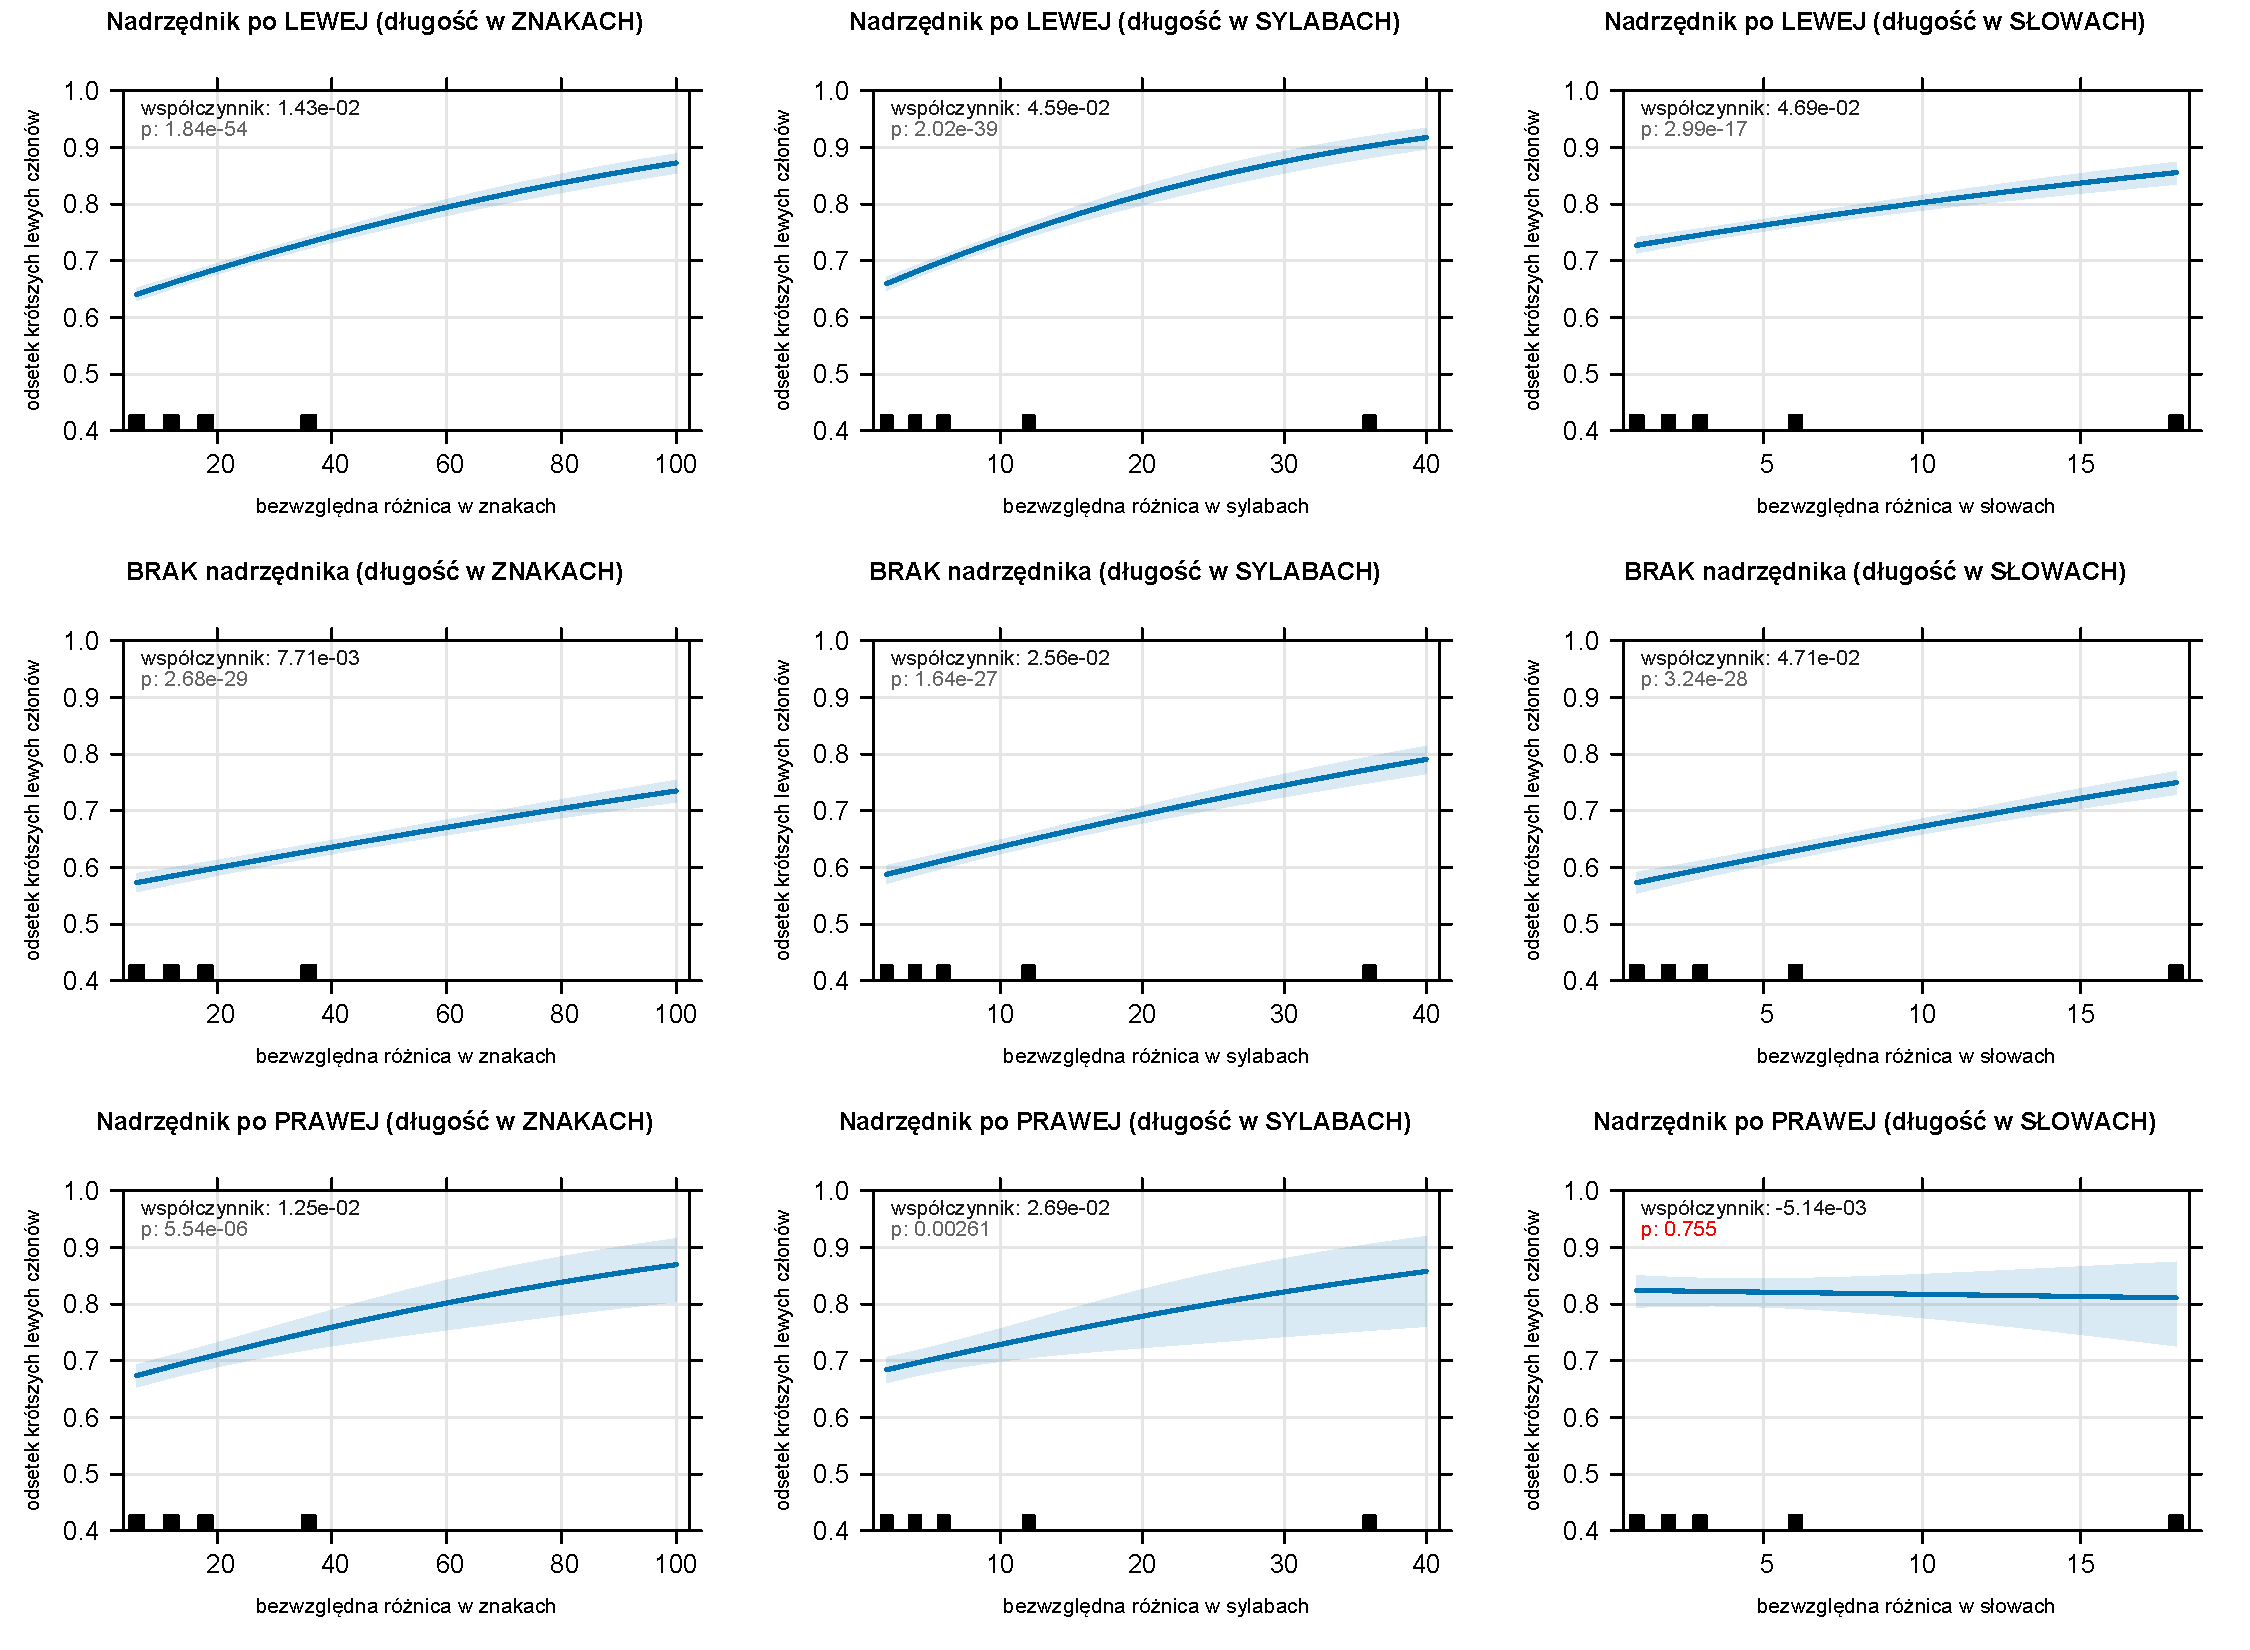
\includegraphics[scale=0.6]{English.pdf}
\caption{Różnica długości członów a występowanie krótszego członu po lewej stronie -- język \textbf{angielski} (\textbf{inicjalny, germański})}
\label{fig:angielski}
\end{sidewaysfigure}

\begin{sidewaysfigure}
\centering
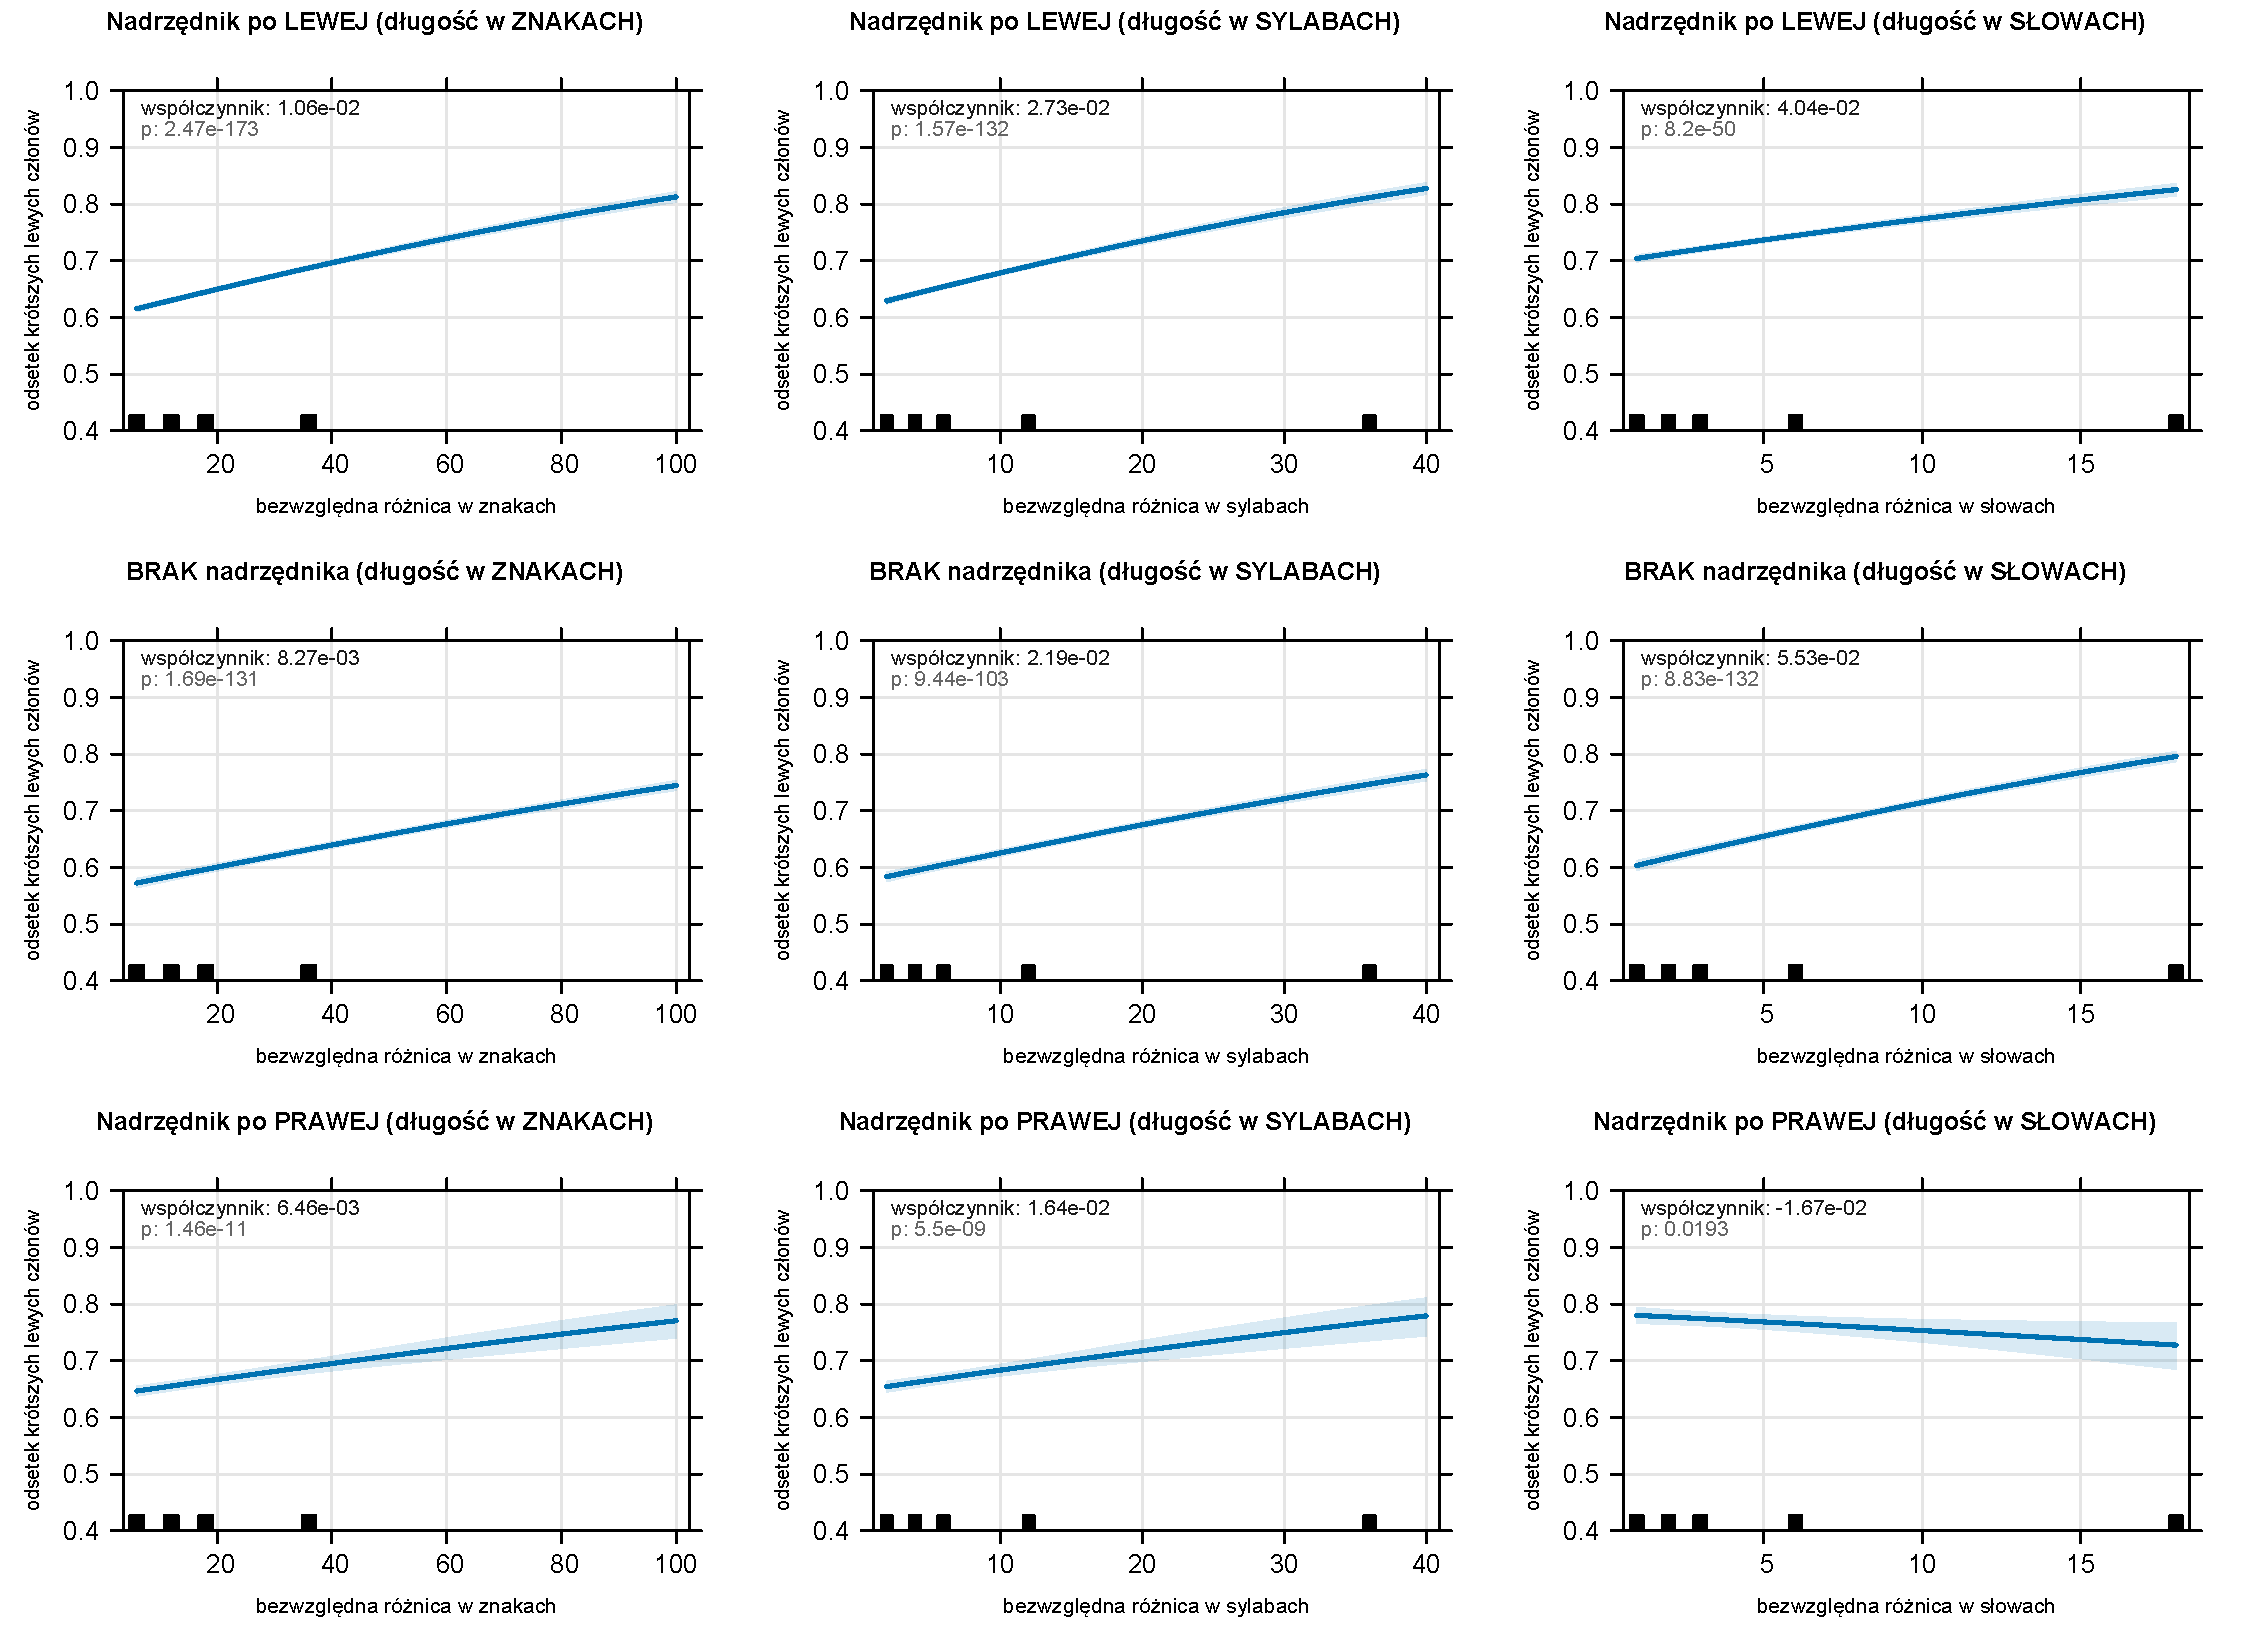
\includegraphics[scale=0.6]{Czech.pdf}
\caption{Różnica długości członów a występowanie krótszego członu po lewej stronie -- język \textbf{czeski} (\textbf{inicjalny, słowiański})}
\label{fig:czeski}
\end{sidewaysfigure}

\begin{sidewaysfigure}
\centering
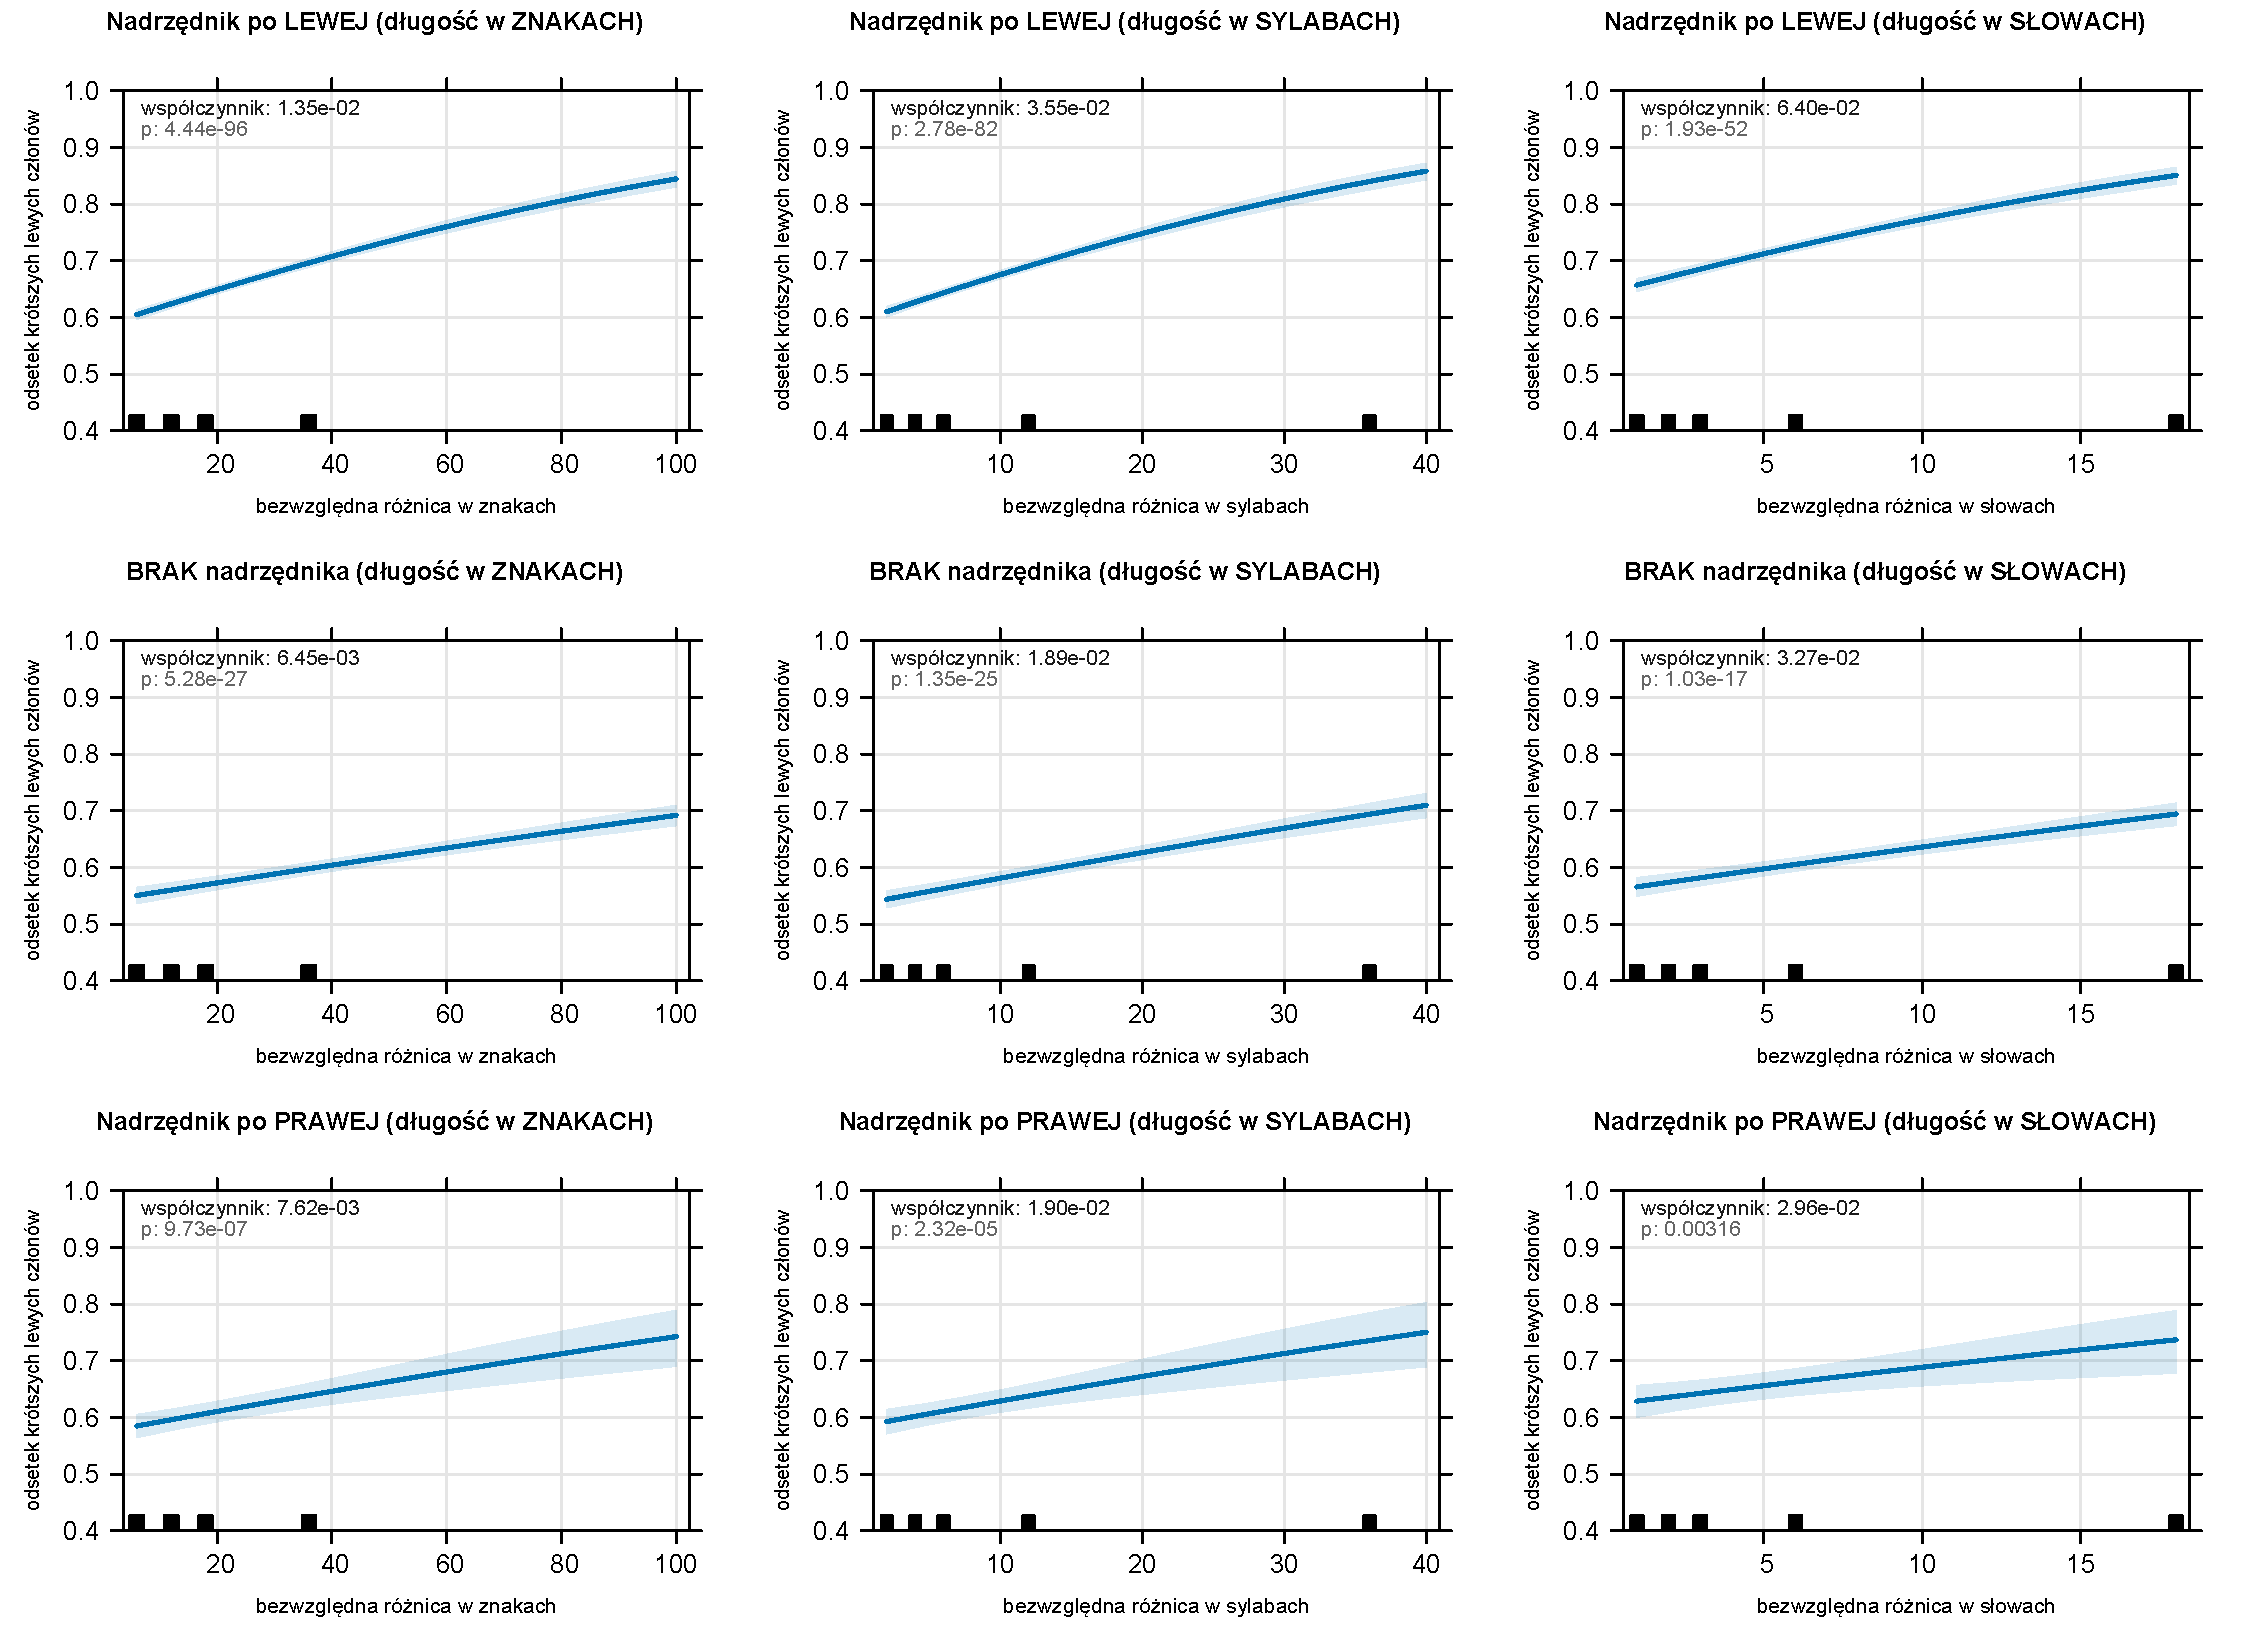
\includegraphics[scale=0.6]{Portuguese.pdf}
\caption{Różnica długości członów a występowanie krótszego członu po lewej stronie -- język \textbf{portugalski} (\textbf{inicjalny, romański})}
\label{fig:portugalski}
\end{sidewaysfigure}

\begin{sidewaysfigure}
\centering
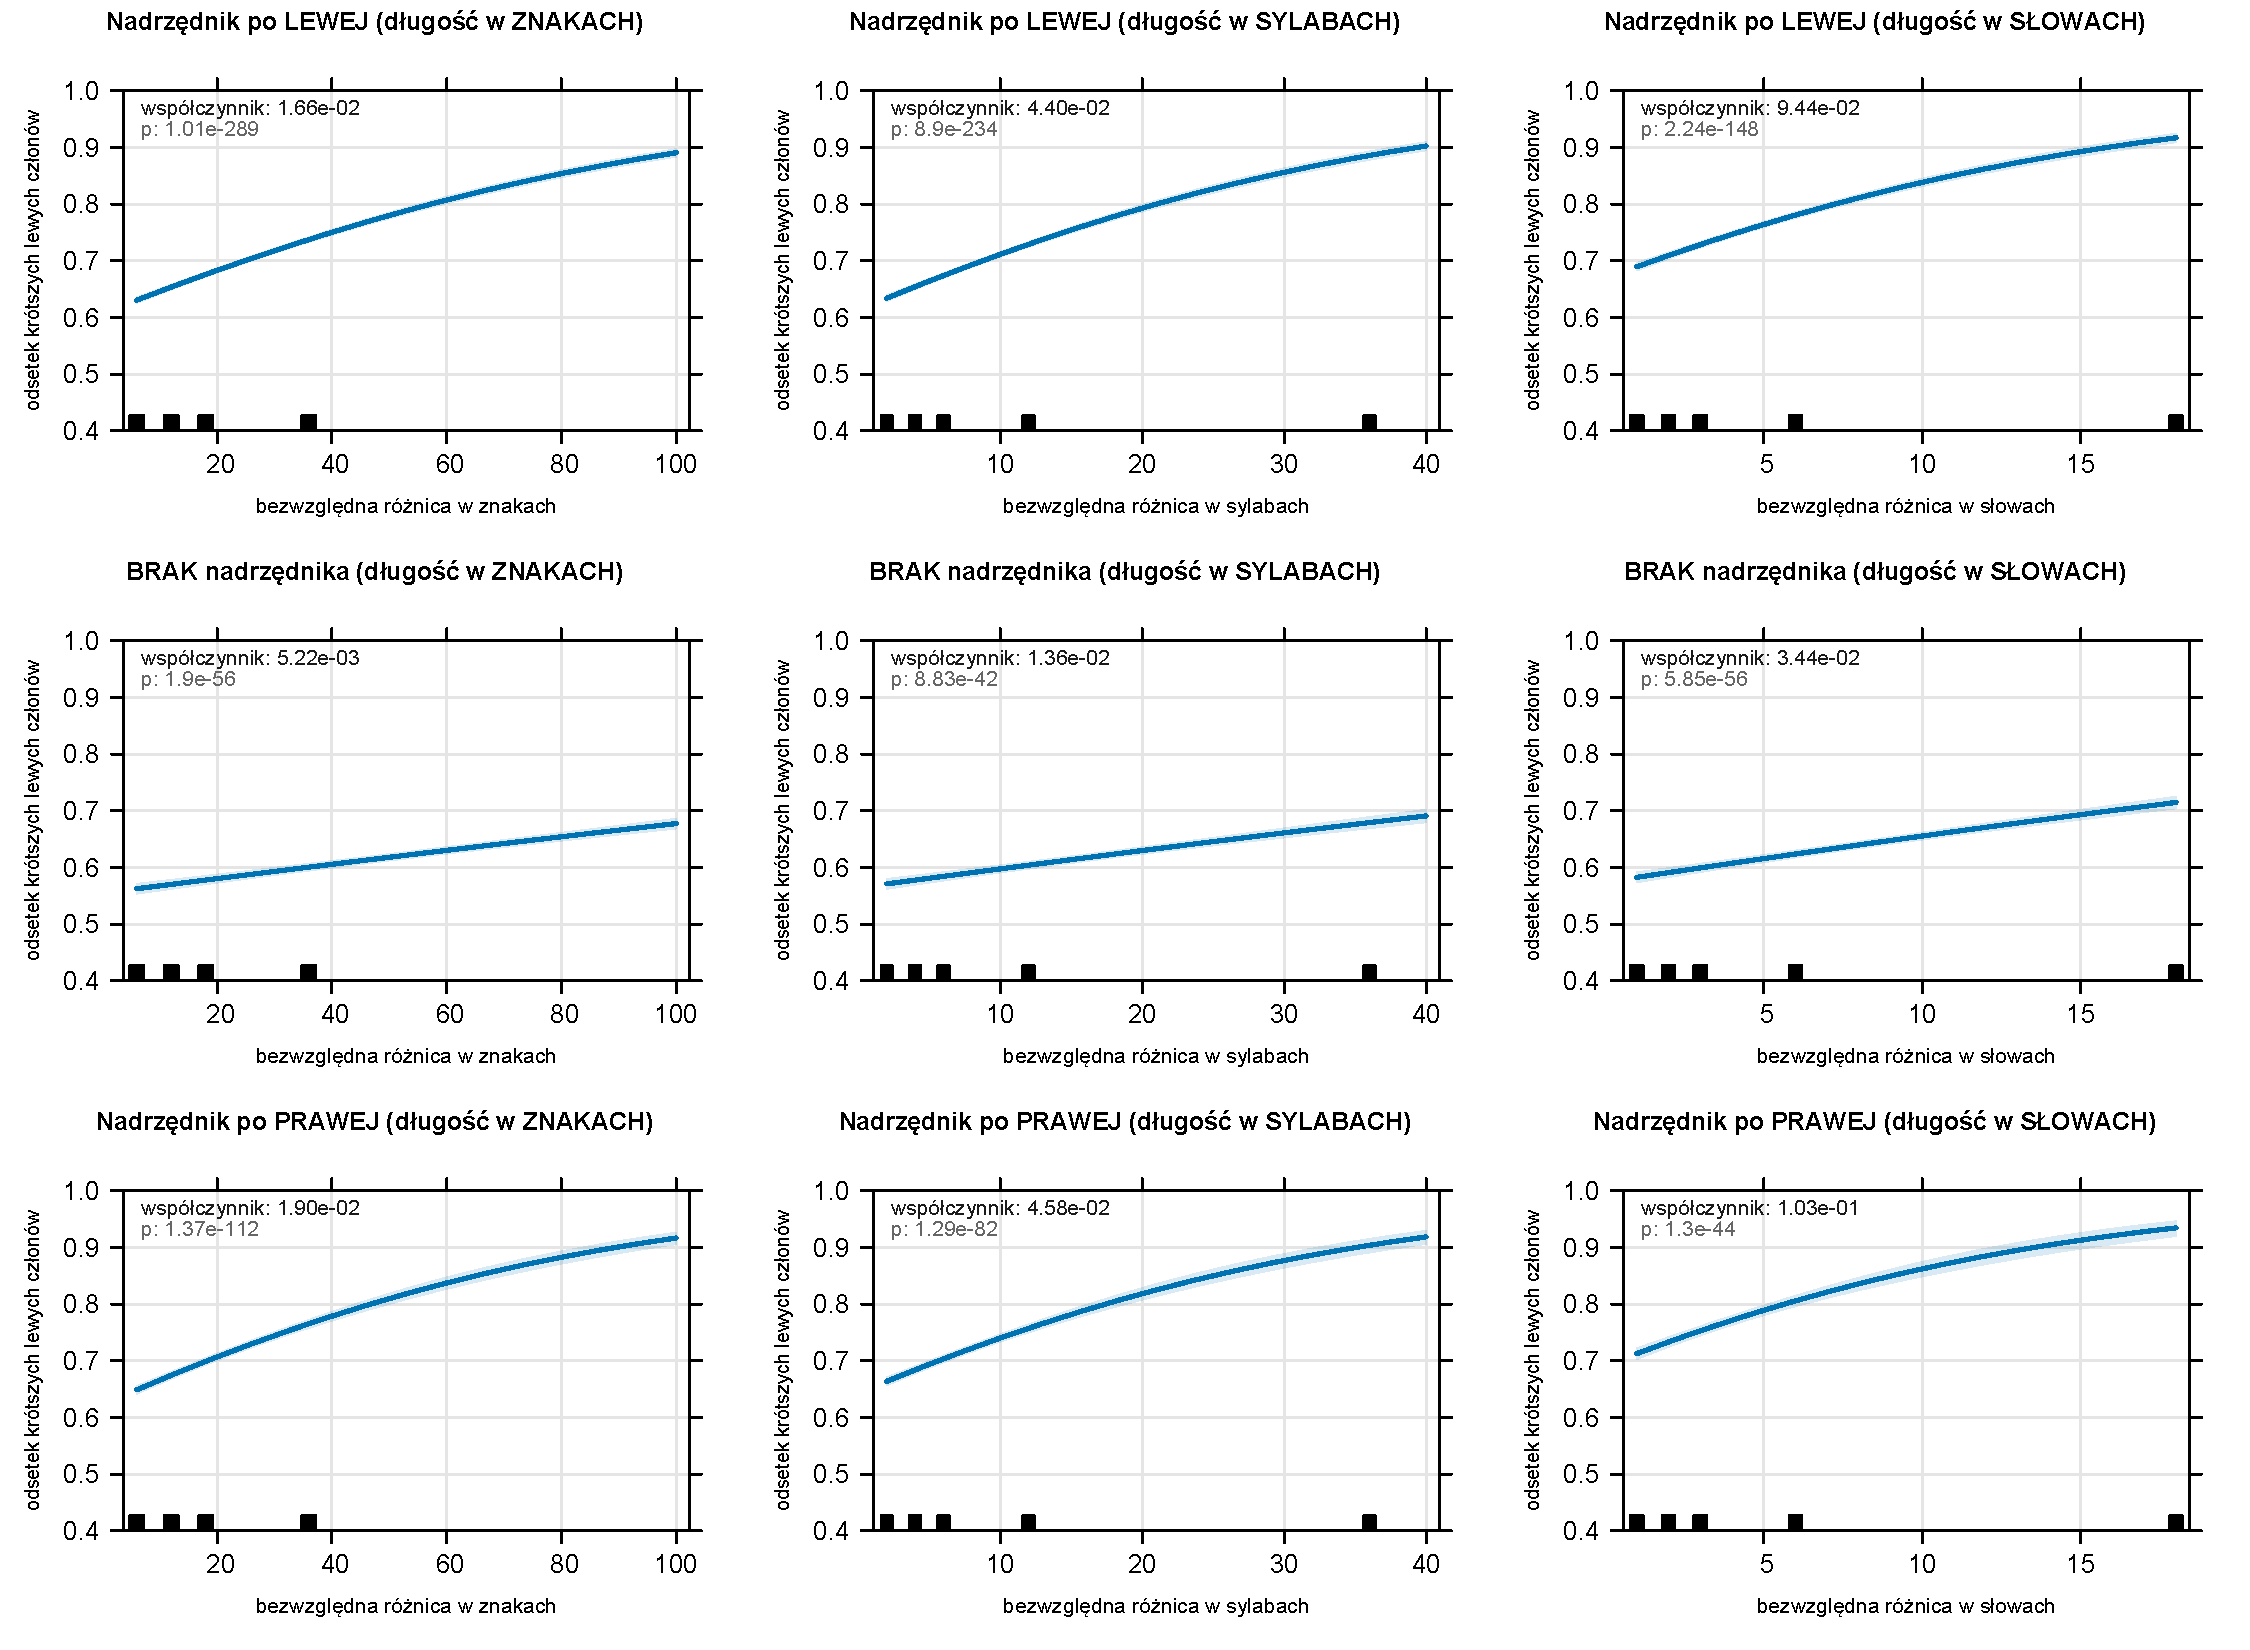
\includegraphics[scale=0.6]{German.pdf}
\caption{Różnica długości członów a występowanie krótszego członu po lewej stronie -- język \textbf{niemiecki} (\textbf{mieszany})}
\label{fig:niemiecki}
\end{sidewaysfigure}

\begin{sidewaysfigure}
\centering
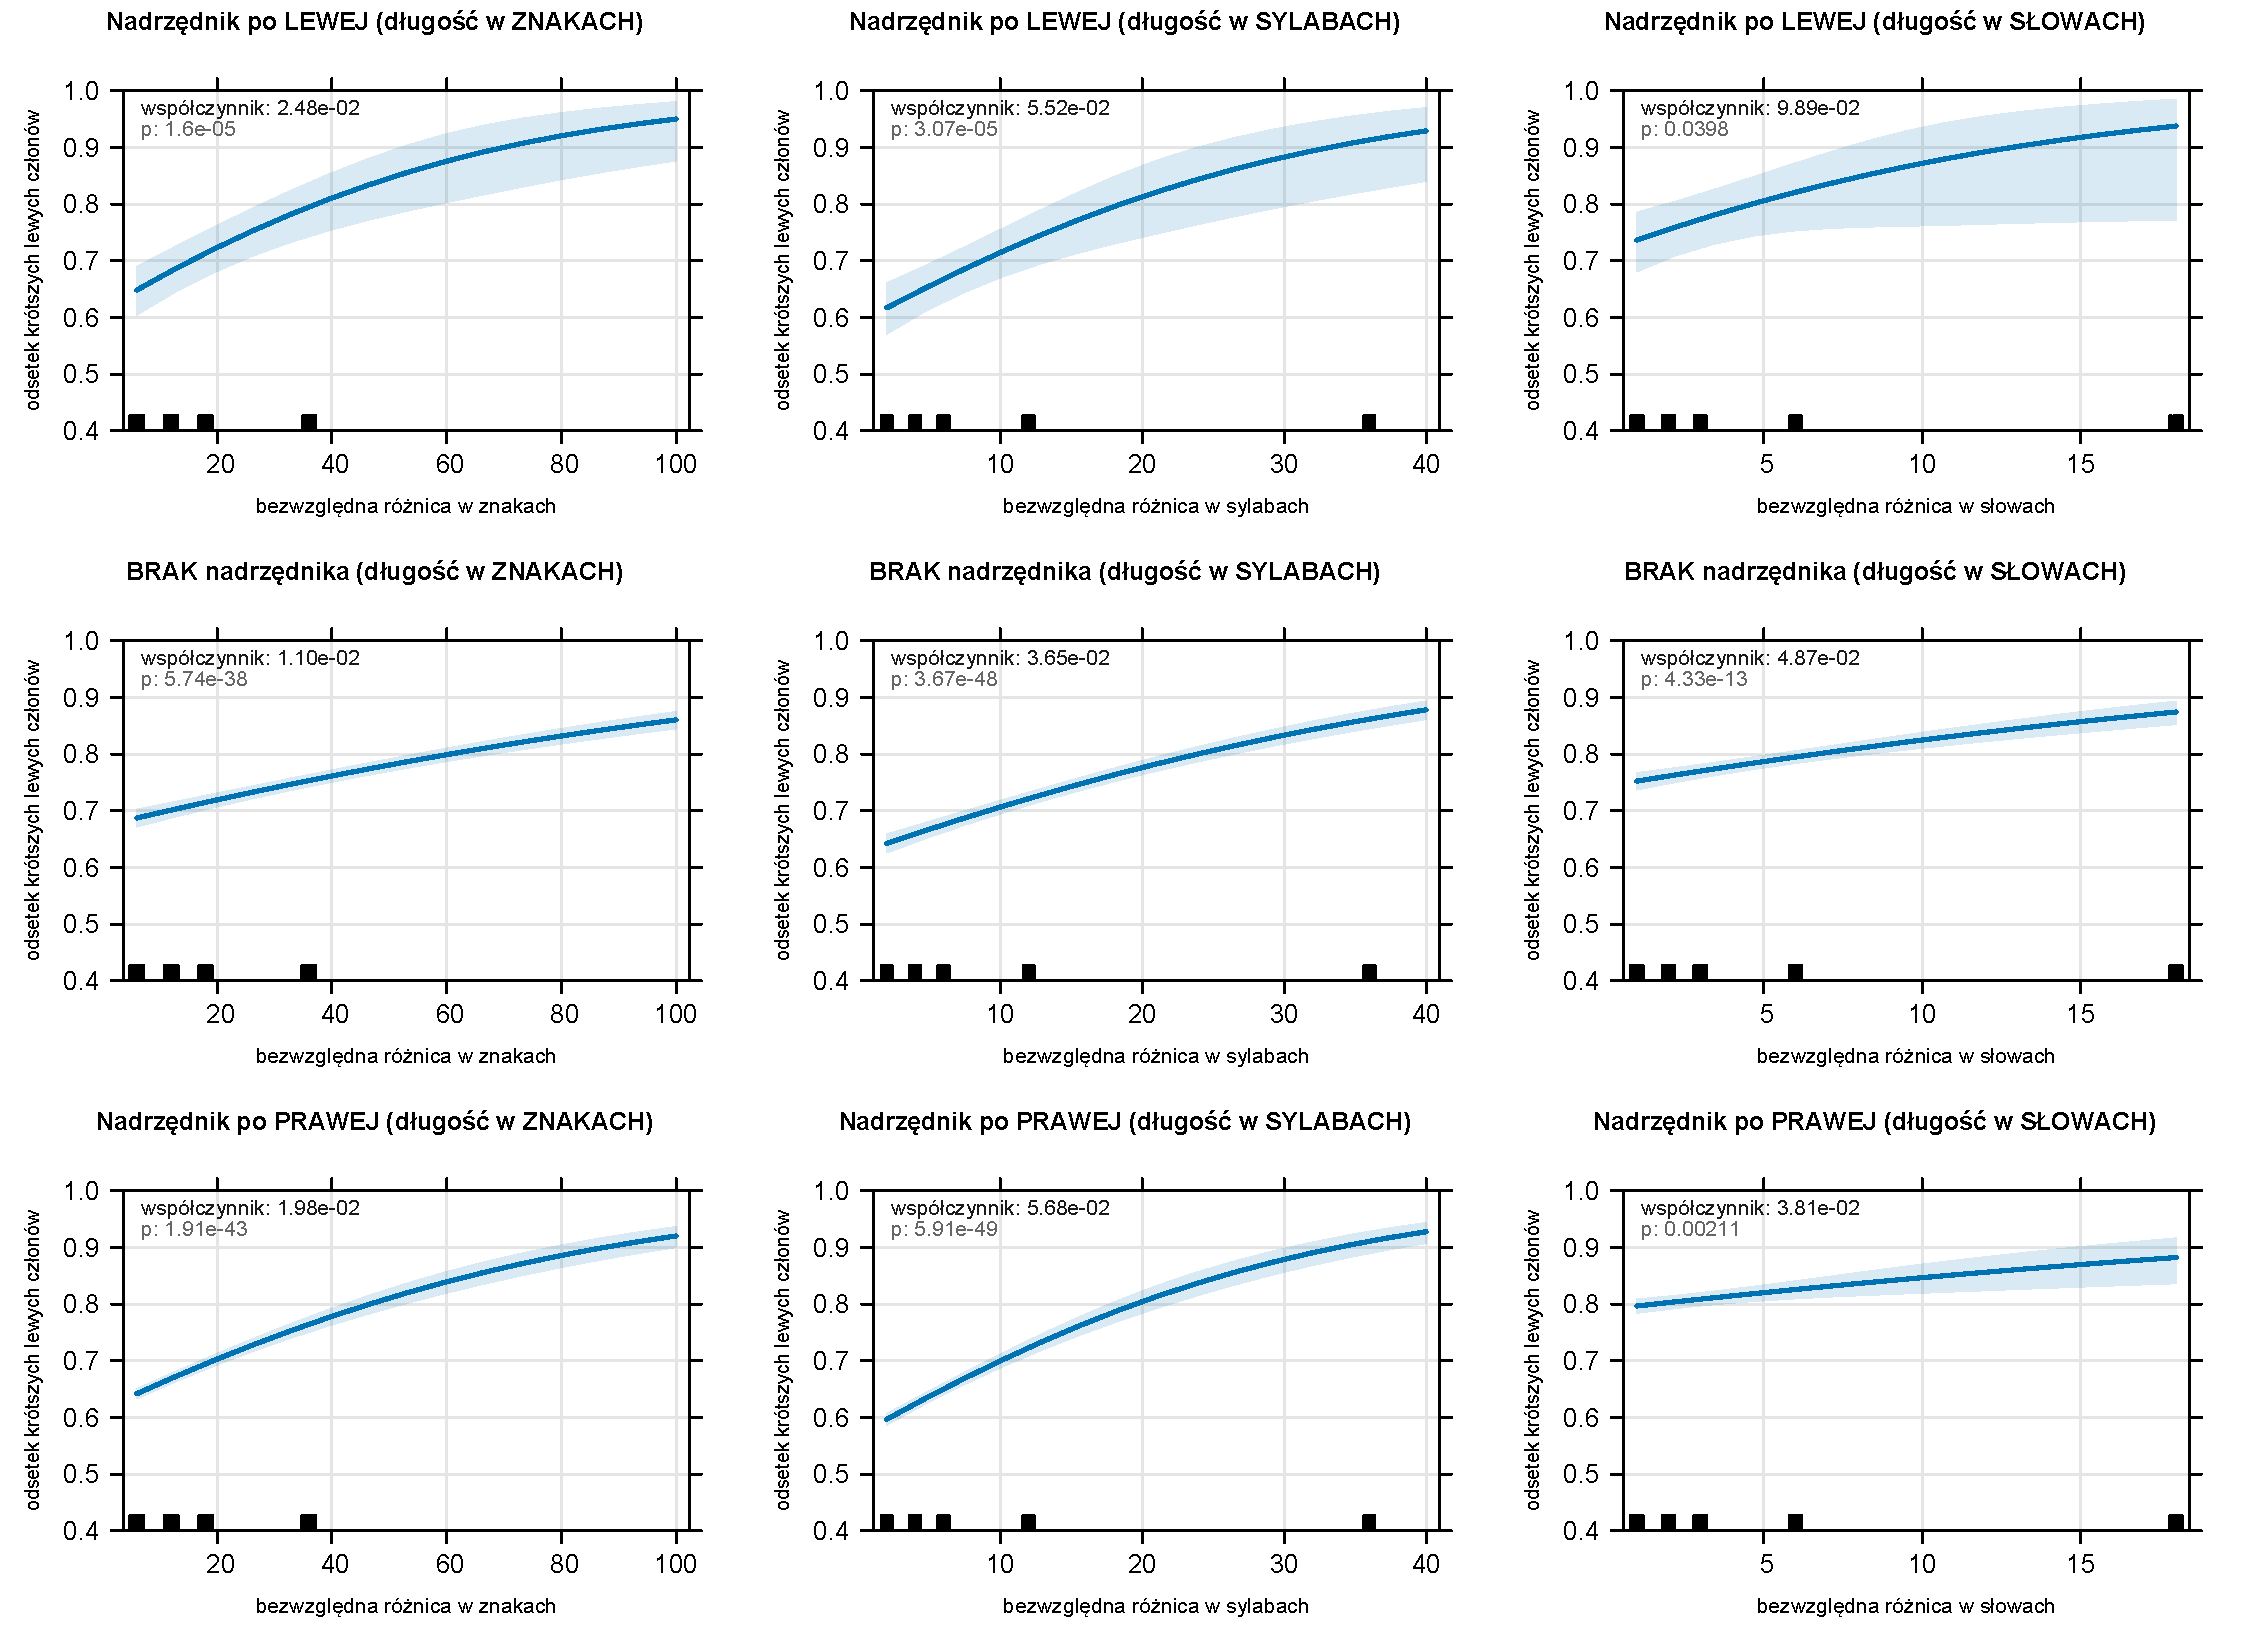
\includegraphics[scale=0.6]{Korean.pdf}
\caption{Różnica długości członów a występowanie krótszego członu po lewej stronie -- język \textbf{koreański} (\textbf{finalny})}
\label{fig:koreański}
\end{sidewaysfigure}